% !TEX root =  CurvedFoldedDogs.tex


\section{Introduction}
There are infinitely many ways to deform a planar sheet without stretching or tearing it. One can either bend it, form sharp creases by folding it, or combine the two. Folding and bending isometries are different by nature, and historically there has been a dichotomy in the study of the two. Smooth bending deformations are typically studied in differential geometry \cite{do_carmo}, whereas straight folds are  explored in the field of computational origami \cite{origami_book}. Curved folded surfaces \cite{huffman} (\figref{fig:teaser}) can be viewed as a combination of the two, since folding an inextensible sheet along a curve necessitates global bending around the crease. These elegant geometries have garnered the attention of architects, artists, and industrial designers \cite{arch_geom,tachi2013composite,tachi2011one,buri2011curved,robofold,curved_review}.

The design of a curved folded surface is manual and time consuming and is usually done using an empirical trial and error approach \cite{curved_review,huffmann_reconstructing}. The known theory on curved folds is confined to a narrow set of folds, and contrary to classical origami, bending and folding instructions are hard to write down and multiple creases must be folded simultaneously \cite{StringActuated:2017}. Artists generally pre-crease the paper using a ball burnisher or a CNC plotter before carefully folding and bending, making the process of shape exploration even slower. 

Although manual and slow, playing with paper is still the predominant approach for curved folded surface design. Existing works on modeling such surfaces are either limited to previously discovered surfaces \cite{curved_folding_kilian,StringActuated:2017} or model a small, partial set of folded surfaces generated by reflections or rotational sweeps \cite{Mitani_ref,mitani2009design}. Modeling the folding process of novel forms remains a challenge \cite{curved_review}. 

In this paper we set out to develop the basic tools for freeform modeling of curved folds, with the objective of aiding the exploration, analysis and study of new curved folded surfaces. Our work builds upon discrete orthogonal geodesic nets (DOGs) \cite{rabi18,rabi2018shape} as a discrete model for $C^2$ developable surfaces. DOGs are regular quadrilateral meshes where around each vertex all angles are equal. Unlike other computational models for developable surfaces, DOGs do not suffer from locking of various deformation modes \cite{locking1,locking2,grin_shells}, \newt{are not limited by an initial choice of meshing or rulings} \cite{pottmann_new,curved_folding_kilian,stein_dev,solomon} (see \figref{fig:rulings_problem_curve}) and do not require remeshing while deforming the surface \cite{StringActuated:2017,SchreckEG2017,Narain}. \newt{Therefore DOGs are particularly suited for modeling curved folds.}
Given an input crease pattern, we represent a curved folded model as a collection of DOGs, with boundary constraints enforcing equal discrete geodesic curvature along their intersections, as done in \cite{rabi2018shape}.

In practice, deforming a set of DOGs while keeping the geodesic boundary constraints does not usually result in a model that is folded along all creases (see \figref{fig:folded_and_not_folded}). Part of the difficulty of modeling these deformations stems from the need to fold all curves simultaneously starting from a flat configuration. \newt{The primary goal of our work is to deal with this difficulty.} 

\subsection{\newt{Contributions}}
\begin{itemize}[label={--}]
  \item \newt{We present a discrete binary characterization for folds between discrete developable surfaces based on supporting planes along creases, motivated by a novel analysis on curved folded surfaces \OSH{do you mean \emph{smooth} surfaces? You analysis is on smooth, then you apply it to discrete, right?}.}
  \item \newt{We use the previous derivation to devise an optimization algorithm capable of enforcing folds while deforming a piecewise DOG, without requiring any folding angles or mountain/valley assignments as input.}
  \item \newt{We further derive optional objectives to control dihedral angles and mountain/valley assignments along folds.}
\end{itemize}
\newt{Though we use DOGs as an underlying model for developable surfaces, our work and derivations can be applied on top of other discrete models for developable surfaces such as ruling based models \cite{conical,curved_folding_kilian,pottmann_new} or models based on discrete shells simulations\cite{grin_shells,shells}.}

%In practice, deforming this set of DOGs while keeping the geodesic boundary constraints does not usually result in a model that is folded along all creases (see \figref{fig:folded_and_not_folded}). Our primary goal is to study deformations that bend as well as \emph{fold} along all creases. Part of the difficulty of modeling these deformations stems from the need to fold all curves simultaneously starting from a flat configuration. \secref{sec:setup} lays the setup for our work, including the problem definition, desiderata and the discrete model we build upon (taken from \cite{rabi18,rabi2018shape}). In \secref{sec:folding} we look at the continuous and combinatorial degrees of freedom of curved foldings, detailing how a flat piecewise smooth developable surface is locally a bifurcation point between folded and unfolded configurations. We discuss how folding along a crease given one side of the surface is a binary choice (see \figref{fig:folding_combinatorics}), give a simple discrete characterization for this choice by looking at supporting planes along the crease and derive objectives to control the basic properties of folding: dihedral angles and mountain/valley assignments. In \secref{sec:implementation} we translate these derivations into an optimization algorithm capable of enforcing folds while deforming a piecewise DOG. Finally, in \secref{sec:results} we model various curved folded surfaces.

\begin{figure} [t]
	\centering
	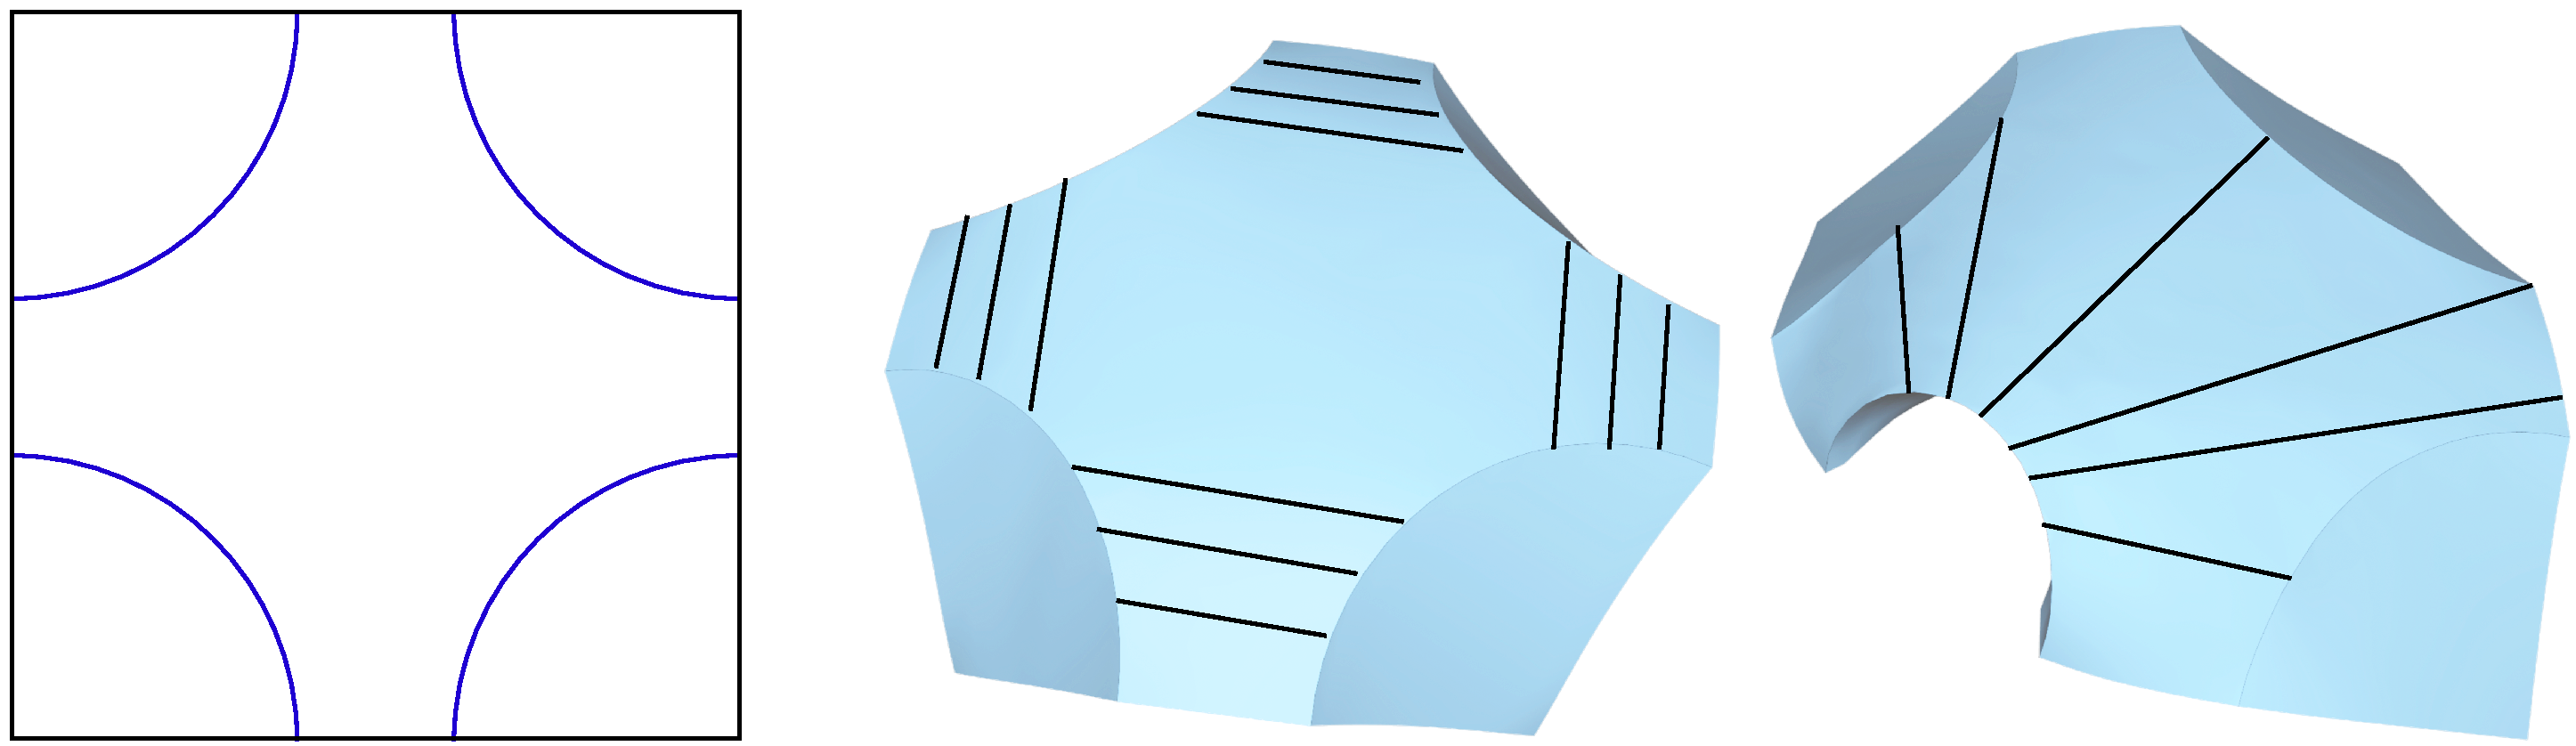
\includegraphics[width=\linewidth]{figures/rulings_problem_curve}
	\caption{Folding and bending the same curved crease pattern (left) into two different surfaces, with some of their rulings plotted. Methods that model the rulings explicitly must remesh in order to model these surfaces, since the rulings can change drastically, connecting vertices of different patches to one another. Representing the curved folded surface as a piecewise DOG avoids the need to remesh because a DOG is parameterized by intrinsic invariants -- orthogonal geodesics -- and does not explicitly encode the developable rulings in its mesh.}
	\label{fig:rulings_problem_curve}
\end{figure}

\begin{figure*} [h]
	\centering
	\includegraphics[width=\linewidth]{figures/fold_bias_compare}
	\caption{Comparison of the same deformation objective with and without our folding algorithm. Up: Crease patterns given as input. Center: Applying a positional based deformation objective of the crease patterns without our folding algorithm results in most crease curves being ignored, i.e. not folded. At this stage, one cannot bend these creases without first flattening the surface. Down: Result of applying the same deformation with our folding algorithm. Our folding algorithm simultaneously folds all crease points while deforming a surface by adding a bias that effectively push flat points towards a folded configuration while not affecting already folded points. The crease mountain/valley assignments, which in these examples are in fact fixed given one choice, are determined automatically without any input. The objective of all of these deformations were the same positional constraints defined on mesh vertices or on a part of a crease curve based on a \textit{curve-constraining flow} \cite{rabi2018shape}.}
	\label{fig:folded_and_not_folded}
\end{figure*}